\documentclass{chi2009}
\usepackage{times}
\usepackage{url}
\usepackage{graphics}
\usepackage{color}
\usepackage{wrapfig}
% \usepackage{picins}
% \usepackage{floatflt}
\usepackage[pdftex]{hyperref}
\hypersetup{%
pdftitle={Browsing the Web of Factual Claims},
pdfauthor={Beth Trushkowski and Rob Ennals},
pdfkeywords={CSCW, sensemaking, web, browsers, collaboration, mind mapping},
bookmarksnumbered,
pdfstartview={FitH},
colorlinks,
citecolor=black,
filecolor=black,
linkcolor=black,
urlcolor=black,
breaklinks=true,
}

\newcommand{\todo}[1]{}
% \newcommand{\todo}[1]{\footnote{{\bf TODO:} #1}}
\newcommand{\Intel}{Intel\textsuperscript{\textregistered}}

\newcommand{\idea}[1]{{\color{blue} IDEA: #1}\\}
\newcommand{\studyresult}[1]{{\color{red} STUDY RESULT?: #1}\\}
\newcommand{\howmany}{{\color{red} (HOW MANY?)}}

\pagenumbering{arabic}  % Arabic page numbers for submission.  Remove this line to eliminate page numbers for the camera ready copy


\begin{document}
% to make various LaTeX processors do the right thing with page size
\special{papersize=8.5in,11in}
\setlength{\paperheight}{11in}
\setlength{\paperwidth}{8.5in}
\setlength{\pdfpageheight}{\paperheight}
\setlength{\pdfpagewidth}{\paperwidth}
%
\toappear{Submitted for review to CHI 2009.}

\title{Browsing the Web of Factual Claims}

\numberofauthors{2}

\author{
	\alignauthor Authors anonymized for submission
}

%\author{
%\alignauthor Beth Trushkowsky\\
%       \affaddr{Computer Science Division}\\
%       \affaddr{University of California at Berkeley}\\
%       \email{trush@berkeley.edu}
%\alignauthor Rob Ennals\\
%       \affaddr{Intel Research}\\
%       \affaddr{2150 Shattuck Avenue}\\
%       \affaddr{Penthouse Suite}\\
%       \affaddr{Berkeley, CA 94704, USA}\\
%       \email{robert.ennals@intel.com}
%}

\sloppy 

\maketitle

\begin{abstract}

Conventional web browsers allow a user to look at pages and follow links between them; however when a user browses the web it is often not the pages themselves that they are looking for but claims about the world that are contained on those pages. A page may contain claims that are contradicted by other pages, or contain one interesting new claim hidden in a sea of claims that the user has already read. If a user is to form an accurate opinion about a topic then they may have to spend considerable time gathering information from many disconnected pages scattered across the web.

We present Think Link, a tool that overlays a network of factual claims on top of the existing web. If a snippet of text on a web page makes a factual claim then a user can use Think Link to connect that snippet to other places on the web that make related claims. We argue that this allows users to more easily find information that will help them understand a topic, evaluate whether a claim is true, and see the range of opinions expressed on the web.

\end{abstract}

\keywords{CSCW, sensemaking, web, browsers, collaboration, mind mapping} 

\category{H.5.2}{Information Interfaces and Presentation}{User Interfaces}[Graphical User Interfaces]

\section{Introduction}

The web provides users with a huge number of pages that they can read, but extracting useful and reliable information from these pages can be difficult. Not everything on the web is accurate~\cite{bbcwebwarning}. If a user is to avoid being mislead by false claims then they will need to either stick to sources they can trust, or spend time looking for evidence on other web sites that supports or opposes what they have read. Similarly, a user will not find every claim on the web interesting. If a user is to locate claims that help them answer the questions they are interested in then they may have to spend considerable time reading claims that do not interest them in order to pick out those that do. Throughout this paper we will use the motivating example of a user who is worried about global warming and wants to find out what is going on and what they can do to help. Many web pages contain claims about global warming that are false, and many web pages repeat the same claims, making it difficult for a user to find interesting new facts that they were not previously aware of.

\begin{figure}[tb]
	\begin{center}
	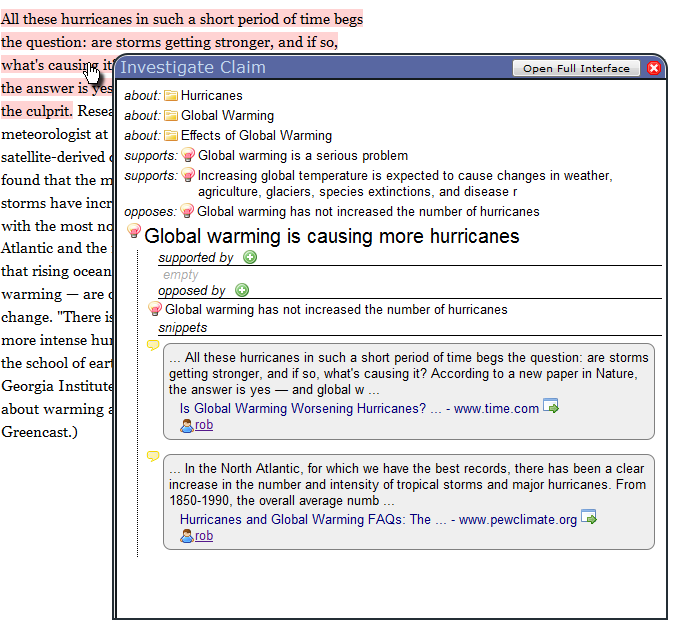
\includegraphics[width=6cm]{../screenshots/claim_popup_crop2.png}
	\caption{Click on a claim to investigate evidence for and against it}
	\label{claimview}
	\end{center}
\end{figure}

The difficulty of finding correct information on the web has been discussed a lot recently. Tim Berners Lee has expressed concern about the difficulty that people face discerning whether information on the web is true~\cite{bbcwebwarning}. Many people have also voiced concerns about how easily people can subvert Wikipedia to give peolpe false information~\cite{wikifalse}. Several commentators have observed that there is a Media Echo Chamber effect~\cite{echochamber,echochamber2} in which news sources report claims that they have heard from other news sources, despite the fact that these claims may be misleading or untrue. If a user only reads news sources from a particular group then they may only be exposed to the views of that group and may not be aware that opposing views exist unless they actively seek them.  

Part of the problem is that conventional web browsing tools require the user to browse by looking at pages, when it is often not the pages themselves that the user is interested in but the factual claims contained within them. While a web page will typically contain links to other articles, these typically only reference a small proportial of the other pages that discuss the topic, and are unlikely to include sources that disagree with the author. The best arguments supporting or opposing a claim may be distributed across a large number of disconnected pages, making it difficult for a user to assemble an argument from the pages on the web. The root of the problem is that the web is structured around where knowledge is coming from (pages written by particular authors) rather than what knowledge is about (the ideas contained on the pages). While this makes it easier for add knowledge to the web, it makes it hard for users to collate all the knowledge available on a topic.


In this paper we present Think Link, a tool that overlays a new network of links over the existing web, connecting snippets of text to snippets elsewhere on the web that make related claims. Think Link maintains a central shared ``claim graph'' (Figure~\ref{summarygraph}) containing claims made on the web, their supporting and opposing relationships to each other, and the snippets that make these claims. When a user views a web page, Think Link highlights snippets that have been identified as making factual claims, with the highlight color indicating whether other sources have been found that disagree with the claim. If a user clicks on such a snippet then they will see a ``claim browser'' (Figure~\ref{claimview}) that allows them to see other claims made on the web that support or oppose the claim the snippet makes, and snippets elsewhere on the web that make these other claims. 

The Think Link claim graph is editable by all users, in a manner similar to a wiki. Any user can add new claims, connect existing claims together, and identify snippets on web pages that make specific claims. Collaborative filtering is used to filter out junk or abusive information, while minimizing the danger of politification.

Not everyone will necessarily want a tool like Think Link. Some people may be looking for confirmation of their own points of view rather than information that challenges their beliefs. We hope however that Think Link may be able to make some contribution to helping peolpe find out about other points of view, and help people more easily find the most interest claims about topics they are interested in.

The contributions of this paper are the presentation of a new approach for connecting information on the web, the design of a user interface that makes it easy for users to find claims that support and oppose claims that they read on the web, and a qualitative user study of how participants use such an interface.


\section{Related Work}

Think Link is very influenced by wikis like Wikipedia~\cite{wikipedia}. Like Think Link, wikis allow users to find information organised by topic rather than author and allow users to collaborate together to bring together all the best information about a topic. Wikipedia's greatest strength is arguable also it's greatest weakness. Since anyone can edit Wikipedia, there is always the danger that information one reads may be incorrect~\cite{wikifalse}. Several projects have attempted to address this problem by tracking sources of edits~\cite{wikicorrect,wikicorrect2}, but it is difficult to remove the problem entirely. While good Wikipedia articles will often include references to sources for their claims, following all sources to check up all claims can be laborious. Think Link tries to avoid this problem by linking claims back to the original sources that made these claims. Users can thus use the known trustworthiness of the original sources to judge the reliability of a claim. Another key difference is that Think Link pulls allows users to provide links from the external web into its graph of claims, thus allowing readers to evaluate the truth of claims they read on arbitrary web pages rather than having to restrict their browsing to a single wiki site.

SpinSpotter~\cite{spinspotter} shares Think Link's goal of allowing users to identify misleading and innaccurate information on web pages that they read. If a user sees a section of text that they think is misleading then they can mark it up, causing it to be highlighted when other users view the same page. While Think Link and SpinSpotter both share the goal of letting users mark up snippets that may be inaccurate, they differ in what they let users find out about such snippets. SpinSpotter allows users to give a textual description of why the snippet is spin and a suggested edit that would make it more accurate. ThinkLink instead connects the snippet to its global claim graph, allowing users to quickly access evidence for and against the truth of the claim. There is alos a difference in the nature of what SpinSpotter and Think Link expect users to mark up. Think Link is interested in evaluating the truth of factual claims, while SpinSpotter also interested in identifying biased phrases (e.g. ``tree hugger'').

Other web annotation systems such as ShiftSpace~\cite{shiftspace}, Stickis~\cite{stickis}, SharedCopy~\cite{sharedcopy}, and Diigo~\cite{diigo} allow people to add their own annotations to existing web pages and view annotations written by other people. Common annotations include commenting on perceived inaccuracies, highlighting interesting passages, or linking to other relavent documents. More generally, tools like WBI~\cite{personalweb} and Mash Maker~\cite{mashmaker} allow arbitrary changes to be made to web pages. We are not aware of any such system that links web pages to a graph of factual claims. 

\begin{figure}[tb]
	\begin{center}
	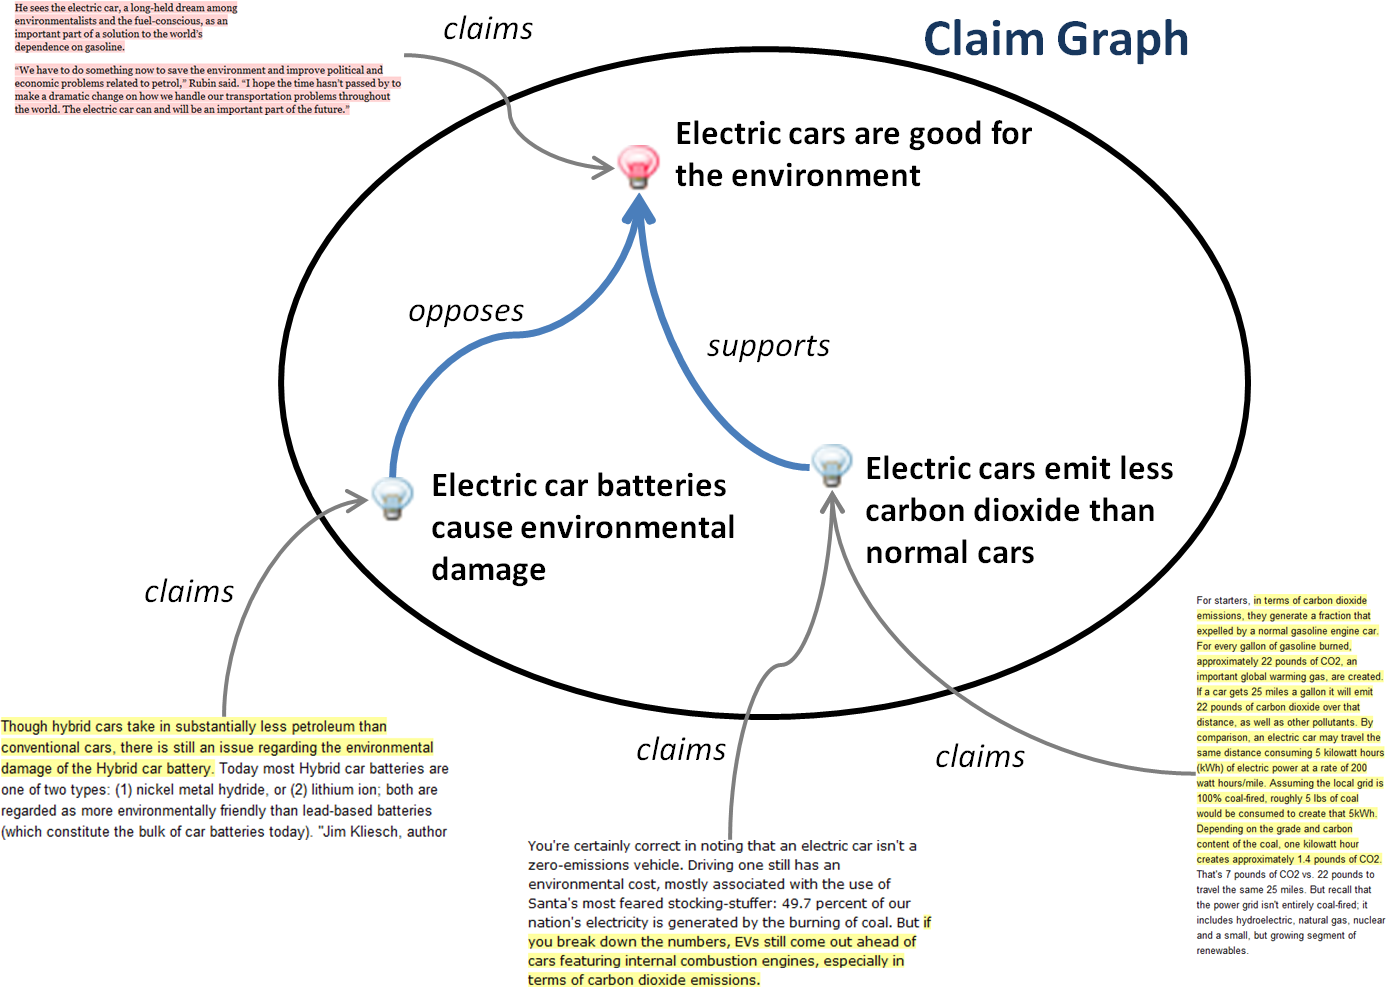
\includegraphics[width=8cm]{../screenshots/summary_graph.png}
	\caption{Think link connects claims to each other and to web snippets}
	\label{summarygraph}
	\end{center}
\end{figure}

Web clipping tools such as Google Notebook~\cite{googlenotebook}, Scrapbook~\cite{scrapbook}, and Zotero~\cite{zotero} allow one to gather and organize interesting from web pages. Many web clipping tools are also web annotation systems.

In Vannevir Bush's seminal MEMEX article~\cite{memex} he proposed an architecture in which links between documents were established by readers, according to the associations between them. As Bush says: ``It is exactly as though the physical items had been gathered together from widely separated sources and bound together to form a new book''. Several more recent systems have allowed user to add links to existing pages. ENQUIRE~\cite{enquire} and TrackBack~\cite{trackback} have bidirectional links, allowing one to see the sites that link to a page as well as those that link from it. Everything2~\cite{everything2} links each page to the most popular pages that users viewed at the same time. Think Link's key difference from this work is that it imposes an additional layer of structure, identifying the factual claims that snippets are making.

One of the goals of Think Link is that people should be able to browse information on the web through the ideas being expressed. This is a goal that is shared with several other projects. Kolak and Schilit~\cite{quotations,quotationsdl} finds places where a passage is repeated in several documents (usually a quotation) and allows users to navigate from such a passage to all other documents where that passage is quoted. Idea Navigation~\cite{ideanavigation} uses a natural language parser to identify subject-verb-object assertions in documents and then allows users to search for browse the assertions in a document corpus. ScentHighlights~\cite{scenthighlights} identifies sections of text that you might find interesting and highlights them for you. ScentTrails~\cite{scenttrails} identifies links to documents that you might find interesting and makes them bigger. Unlike Think Link, these tool attempt to extract text of interest automatically, rather than relying on users to identify and connect interesting factual claims.

Much work has been done on the idea of using a graph to represent an argument~\cite{argumentatino,argmas}. Popular argument models include the Toulmin Model~\cite{toulmin}, the Carneades Model~\cite{carneades}, and the IBIS model~\cite{ibis}. Models used for argumentation theory are usually significantly more complex than our simple supports/opposes model, with the result that they provide a more accurate model of the logical argument, at the cost of requiring more skill to assemble. One feature found in some argumentation graphs~\cite{Korb97acognitive} that we may add in the future is the ability to attach a numberical weight (maybe from voting) asserting how much a claim supports or opposes another claim, or how reliable a claim is.


%\subsection{Automated Reasoning}
%
%Case-Based reasoning
%Sensemaking

%\subsection{Argumentation Graphs}
%Argumentation graphs express positions and arguments in a formal graph model as nodes and edges, respectively, and are typically used to make a decision or draw a conclusion about some issue. One example implementation is the {\it Zeno} argumentation framework~\cite{zeno}, designed for collaborative use in mediation systems to debate the quality of alternative solutions for a problem. In their object model of argumentation elements, based on Rittel's IBIS model~\cite{ibis}, example nodes include pro/con arguments, positions, preferences, comments, and decisions. Importantly, arguments are connected via {\it consequent} and {\it antecedent} edges, which are used to inform {\it choices}. The decision-making power of the argumentation graph follows from the traversal of argument relationships to enhance the depth and breadth of understanding about an issue. Our application similarly links claims as {\it supporting} and {\it opposing} other claims to allow users to develop a cohesive understanding of arguments.
%
%Traditional argumentation graphs are designed to solve a specific, isolated issue. Our application supports an ever-expanding set of topics, and arguments can form links between multiple topics. Users can consult the web of ideas directly to form an opinion about a particular issue, but they can also browse for new issues to explore. Opinions or decisions in our model don't have to be static: as the topic is expanded with more supporting and opposing evidence, users may alter previous viewpoints. Another advantage of our model is that the ability to explore claims' source-document evidence is built right into the navigation. Looking at an argument shows both its related argument as well as its supporting {\it snippets}, allowing the user to explore the evidence for himself. 

\section{The Think Link System}


\begin{figure}[tb]
	\begin{center}
	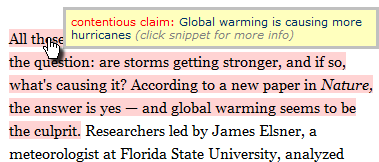
\includegraphics[width=6cm]{../screenshots/highlight_crop.png}
	\caption{Hovering over a highlighted snippet shows a summary}
	\label{highlight}
	\end{center}
\end{figure}


Think Link is a tool that overlays a web of factual claims on the existing web (Figure~\ref{summarygraph}). As a user browses the web, Think Link highlightes snippets of text that have been identified as making factual claims. If a user clicks on a highlighted snippet then Think Link will display an interface that allows the user to easily find snippets on other pages that make related claims (Figure~\ref{claimview}). Our intention is that Think Link allows a user to easily access the best arguments for and against a claim that can be found on the web, and allows users to more easily evaluate the truth of claims that they read.

Think Link has a global graph of factual claims that is shared by all users (Figure~\ref{summarygraph}). This graph is managed like a Wiki, allowing any user to add new claims or snippets. As a user browses the web, they can identify snippets that make claims that are interesting or contraversion and link them into the global claim graph. Think Link is implemented as a FireFox extension~\cite{firefoxextend} and so can be applied to arbitrary websites without requiring them to be aware of Think Link.


\subsection{Exploring factual claims on a page}

When a user browses a web page, we want to make them aware of claims being made on the page that they might find interesting, or that other sources disagree with. Think Link draws attention to the factual claims that other users have identified on a web page by highlighting them (Figure~\ref{highlight}). Snippets are highlighted in red if they are contentious (other sources disagree with the claim). The highlight colors are chosen such as to be pale enough to not impede reading, but dark enough to be noticeable. A user can see what claim a snippet is making by hovering their mouse over the snippet (Figure~\ref{highlight}).

\begin{figure}[tb]
	\begin{center}
	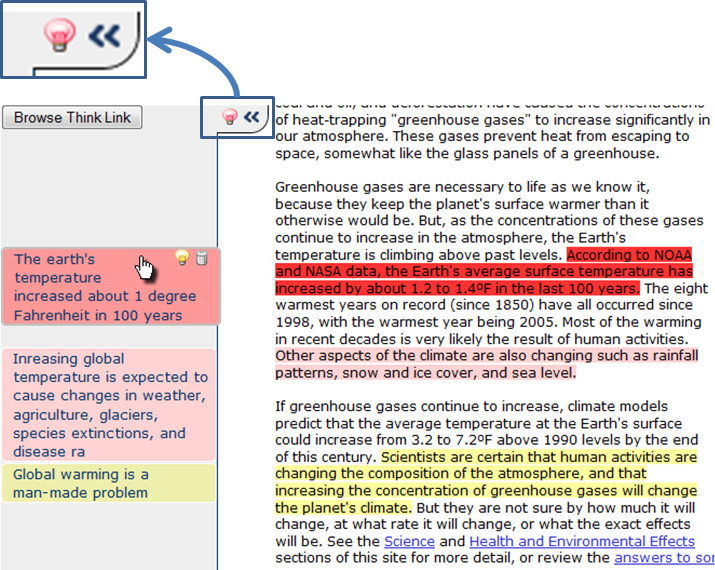
\includegraphics[width=6cm]{../screenshots/sidebar_diagram.png}
	\caption{The margin summarizes the key claims on the page}
	\label{margin}
	\end{center}
\end{figure}

If a user thinks a claim is interesting and wants to know what other sources say about it then they can open up a ``claim browser'' window (Figures~\ref{claimview} and \ref{claimbrowse_diagram}) by clicking on the highlighted snippet. The claim browser allows the user to easily view claims that support or oppose the selected claim, and the snippets of text on the web that make these claims (Figure~\ref{claimview}). 
For example, if a user browsed a web page that claimed ``Global Warming does not exist'', then the snippet that made this claim would be highlighted in red, indicating that there are web pages elsewhere that make opposing claims. If the user were to click on the highlighted snippet then an ``investigate claim'' window would appear. This window would show that the claim ``Global Warming does not exist'' is opposed by the claim ``There is strong evidence for global warming''. If the user navigated to this new claim then they could quickly see the best claims that support the existence of global warming, and would be able to see summaries of the best sources that supported these claims.

%\begin{floatingfigure}{2cm}
%
\includegraphics[width=2cm]{../screenshots/marginpull_out.png}
%\end{floatingfigure}

\begin{wrapfigure}{r}[0.5cm]{2cm}

\includegraphics[width=2cm]{../screenshots/marginpull_out.png}
\end{wrapfigure}
If the current page contains snippets then a tab appears in the top left corner of the window. The tab contains a lightbulb whose color changes according to the nature of the snippets on the page - red if a snippet contains a contentious claim. This allows a user to quickly tell if a page contains something of interest without having to scroll down. Clicking on the tab opens the margin. The margin provides a summary of all the intersting claims that users have identified on the current page and is designed to mimick the traditional margin notes that readers often write on physical documents~\cite{marginalia}. To emphasise the connection between a margin note and its associated snippet, each margin note is aligned vertically with its snippet and the snippet is highlighted more strongly when the user mouses over the associated margin note. 

We found that when a participant sees a highlighted snippet, they will typically want to do one of four things: ignore it, remember it, delete it, or investigate it. If the user finds the snippet interesting and wants to use it later then they can bookmark it by clicking the bookmark icon that pops up when they mouse over the margin note. This will cause it to be displayed prominently in the claim browser. If the user believes the snippet to not be making the claim that it says it does or otherwise badly marked up then they can delete the snippet by clicking on the trash can icon on the margin note. If the user thinks the claim is interesting and wants to see how it relates to claims made by other snippets on the web then they can click on the highlighted text or the margin note to open the claim browser.

\subsection{The Mental Model}

\begin{figure}[tb]
	\begin{center}
	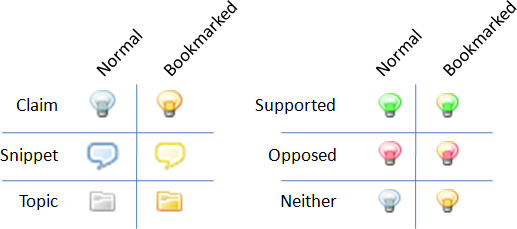
\includegraphics[width=7cm]{../screenshots/bookmark_icons.png}
	\caption{Icons used for Claims, Snippets, and Topics}
	\label{bookmark_icons}
	\end{center}
\end{figure}


Think Link users interact with three kinds of object, each of which is associated with a different family of icons (Figure~\ref{bookmark_icons}): 	

\begin{itemize}
\item {\bf a claim} (
\includegraphics[width=0.3cm]{../images/lightbulb_off.png}) is a factual claim about the world that may be true or false. For example ``Global warming is man made''. A claim may support or oppose other claims. Claims are written as raw English\footnote{though one can imagine supporting other languages in the future} text and Think Link does not try to understand what they mean semantically.
\item {\bf a snippet} (
\includegraphics[width=0.3cm]{../images/comment.png}) is a section of text on a web page that asserts or assumes the truth of a particular claim. Many snippets may assert the same claim and users are encouraged to re-use existing claims rather than creating new ones when creating new snippets.
\item {\bf a topic} (
\includegraphics[width=0.3cm]{../images/folder_grey.png}) is a thing that claims can be about. For example ``Global Warming'', or ``Computer Science''. A claim can have one or more topics that it is about, and a topic can have one or more more general topics. Topics are used both to organize, and to disambiguate claims. For example ``Bush'' can mean either ``George H W Bush'', ``George W Bush'', ``Vannevar Bush'', ``Kate Bush'', ``The Rock Band Bush'', or just ``A Bush''. Associating a claim with a topic allows one to write shorter claims without worrying about being ambiguous.
\end{itemize}

Varients of these three icons are used consistently when refering to these three object types. 
Yellow versions of these icons are used to identify claims, folders, or snippets that the user has marked as interesting (by clicking on their icon). 

Colors are also used to indicate the extent to which a claim is supported or opposed by other claims. Red means that a claim is opposed by other claims, and green means that a claim is supported by other claims and not opposed by any. The colors are chosen to fit with people's normal associations with colors, where red is commonly associated with danger (e.g. a traffic light) and yellow is the standard color used for highlighter pens.


\subsection{Collaborating to connect claims}

Think Link shares a lot in common with Wikis like Wikipedia~\cite{wikipedia}. The claim graph is shared between all users and editable by anyone. Any user can identify a claim made on a web page by selecting the web snippet that makes this claim and clicking the ``new snippet'' button on the browser toolbar. Similarly, any user can establish new supporting and opposing relationships between claims by using drag and drop within the claim browser. One can think of Think Link as being rather like a Wiki in which all the content is clipped from existing sources and links are created from those sources back to the wiki.

Think Link uses collaborative filtering~\cite{collective} to highlight the most interesting claims that support and oppose another claim, and the most interesting snippets that make a claim. If a user finds a snippet or claim interesting then they can mark it as such. When Think Link lists claims or snippets, it will show first those that the user marked as interesting, and order the rest according to the number of other users who marked them interesting.

It is important to avoid political fights, where two competing sides delete claims, snippets, or connections that they disagree with. Similarly, it is important to avoid vandalism, where people abuse people with competing beliefs by adding abuse claims or snippets. While we do not have a perfect solution to this problem, our current approach is to treat deletion as a special case of collaborative filtering. A claim or snippet will only be deleted if many people vote to delete it and very few people bookmark it. 


\subsection{Why People Annotate}

Tools like Think Link rely on user contributions in order to be useful. If no users are identifying factual claims on pages then other people who browse such pages will not see any claims identified. Similarly, if no other users are connecting claims together, then users will not see any supporting or opposing claims when they click on a highlighted snippet.

Moreover, in order to become popular, a tool like Think Link needs to be useful even when very few people are using it. If a tool is only useful when it has a large community using it then it is unlikely that early adopters will stick with it enough for it to ever acquire a large community.

Our user study participants identified several reasons why they would want to mark up factual claims in documents they found. The most common reason people gave for identifying and organizing factual claims was if the person was writing an article or researching a topic and wanted to keep track of the information they had found. One user (who was an active blogger) also expressed an interest in finding and marking up instances of claims that he disagreed with, so that readers would see the arguments highlighted in red and be directed to the counter-arguments. The same user also expressed an interest in marking up claims in documents he had made in his own articles so that readers could quickly see the evidence he had found in support of his claims.


\section{Interaction Techniques}
\label{interface}

Users interact with Think Link in four key ways. Think Link will draw attention to interesting claims on pages that the user browses; it allows the user to identify new factual claims on pages they browse; it allows them to browse the graph of related claims and identify the strongest evidence supporting or opposing the claims they are looking at; and it allows them to organize the claim graph by making new connections between existing claims and topics.


\subsection{Browsing factual claims}
\label{browseclaim}\label{claimbrowser}

\begin{figure}[tb]
	\begin{center}
	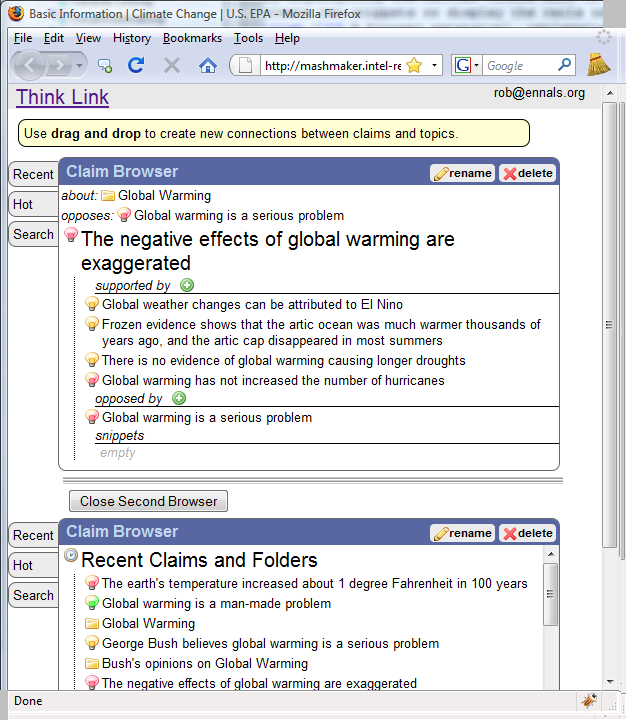
\includegraphics[width=6cm]{../screenshots/claimbrowse.png}
	\caption{The Claim Organizer contains two claim browsers}
	\label{fig:claimbrowser}
	\end{center}
\end{figure}

\begin{figure}[tb]
	\begin{center}
	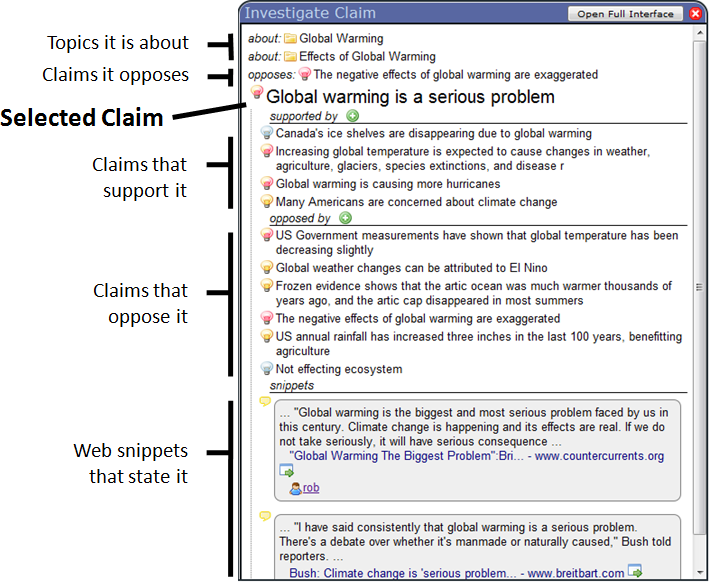
\includegraphics[width=8cm]{../screenshots/claimbrowse_diagram.png}
	\caption{The Claim Browser Allows one to browse the argument graph}
	\label{claimbrowse_diagram}
	\end{center}
\end{figure}
\begin{figure}[tb]
	\begin{center}
	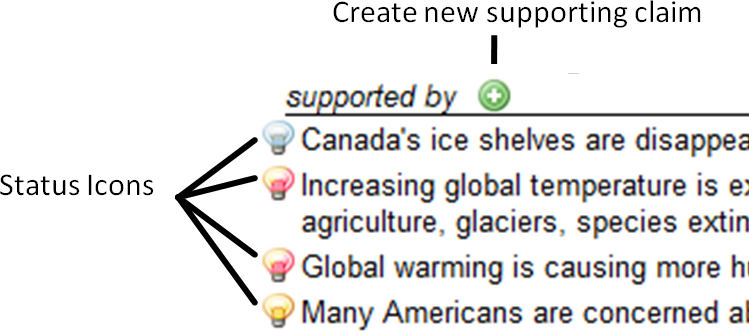
\includegraphics[width=8cm]{../screenshots/claimbrowse_zoom.png}
	\caption{Close up of a list of supporting claims}
	\label{claimbrowse_zoom}
	\end{center}
\end{figure}

\begin{figure}[tb]
	\begin{center}
	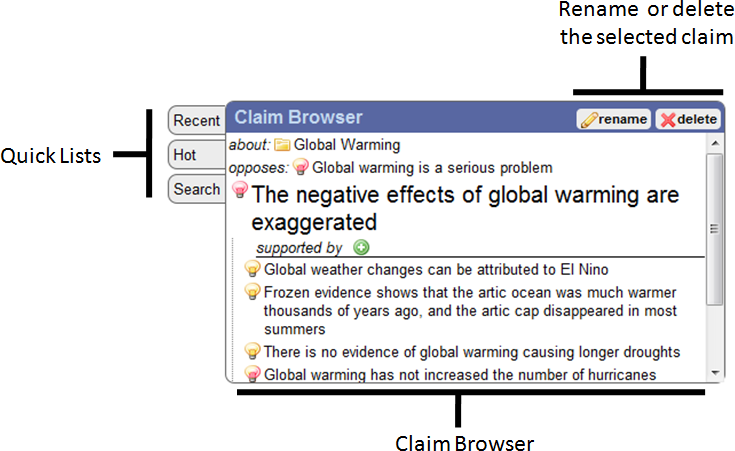
\includegraphics[width=8cm]{../screenshots/fullbrowser.png}
	\caption{The Enhanced claim browser adds additional controls}
	\label{enhancedbrowser}
	\end{center}
\end{figure}

Our users expressed an interest in using snippets to help them construct arguments that support a claim they agree with, to show them the arguments for and against a claim that they are unsure about, to collect evidence about a topic they are interested in, to share information with friends, and to see arguments against claims that they encountered on the web. We constructed the ``claim browser'' interface to help users do these things (Figure~\ref{fig:claimbrowser}).

Claims and topics form a directed graph structure. A claim can have any number of claims that support or oppose it, and any number of claims that it supports or opposes.
A topic can have any number of more specific topics (e.g. ``US Election 2008'' is more specific than ``US Elections'') and any number of more general topics. A topic can also have any number of claims about that topic.

When designing an interface to this structure, we were faced with two opposing constraints. We needed to be able to clearly view a large number of claims and topics in a small screen space, and we needed an interface that made it clear that the data was a graph rather than a tree. Dynamically reorganizing graphs such as those used in Vizster~\cite{vizster} and Personal Brain~\cite{thebrain} made the graph structure very clear, but made it difficult to clearly view large numbers of claims. Tree-based outliners such as OmniOutliner~\cite{outliner} made it easy to view large numbers of related claims, but made it difficult to present an impression of the data being a graph rather than a tree.

\todo{This interface is actually closer to TheBrain than the text suggests}

After several iterations, we settled on an interface that is a dynamically reorganizing graph layed out like an outliner. Like other dynamically reorganizing graphs, the interface is arranged around the currently selected node, and when a new node is selected the interface animates to surround the newly selected node with objects to relate to it. Like an outliner, the nodes that relate to the selected node are listed vertically below the selected node, each on their own line. Our users commented that they found it quite intuitive to navigate through a graph of claims and topics in this way. \studyresult{quote}.

The placement of objects above and below is intended to emphasize the conventional structuring of an argument graph, with topics going upwards and arguments for and against a claim going downwards. A user can navigate down to get to explore why a claim may or may not be true, or navigate up to find out about more general topics, or claims that the selected claim supports or opposes.

\todo{Have I seen an interface like this elsewhere? Did PARC have something like this?}

\todo{Is this interface a contribution in itself? Has an interface like this been presented before?}

Animation is used throughout the interface to give users a sense of where they are and how the current interface state related to previous states. When a new item is selected, it grows in size and moves to the center. Other items that were already on the screen move from their current locations to their new locations. Other objects appear and disapper by smoothly sliding into or out of view. We found that this animation helps users retain a sense of where they are with respect to what they were looking at previously and helps users avoid getting lost.

Users see a claim browser in three different places:
\begin{itemize}
\item {\bf The Main Organizer} shows two claim browsers, and allows users to use drag and drop to make new connections between claims in the two organizers. (Figure~\ref{fig:claimbrowser})
\item {\bf The Popup Browser} shows one claim browser in a reduced-size window and is used to quickly investigate a claim found on a web page. (Figure~\ref{claimview})
\item {\bf The Claim Selection Window} shows one claim browser, together with the text of a new snippet, and is used to identify the claim that a snippet is making. (Figure~\ref{snipsavecrop}) 
\end{itemize}


\subsection{Identifying new factual claims}
\label{newsnippet}

\begin{figure*}[tb]
	\begin{center}
	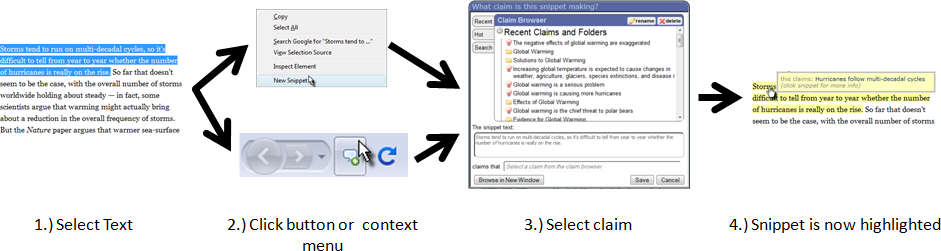
\includegraphics[width=16cm]{../screenshots/newsnip_all.png}
	\caption{Process for creating a new snippet}
	\label{createprocess}
	\end{center}
\end{figure*}

%\begin{figure}[tb]
%	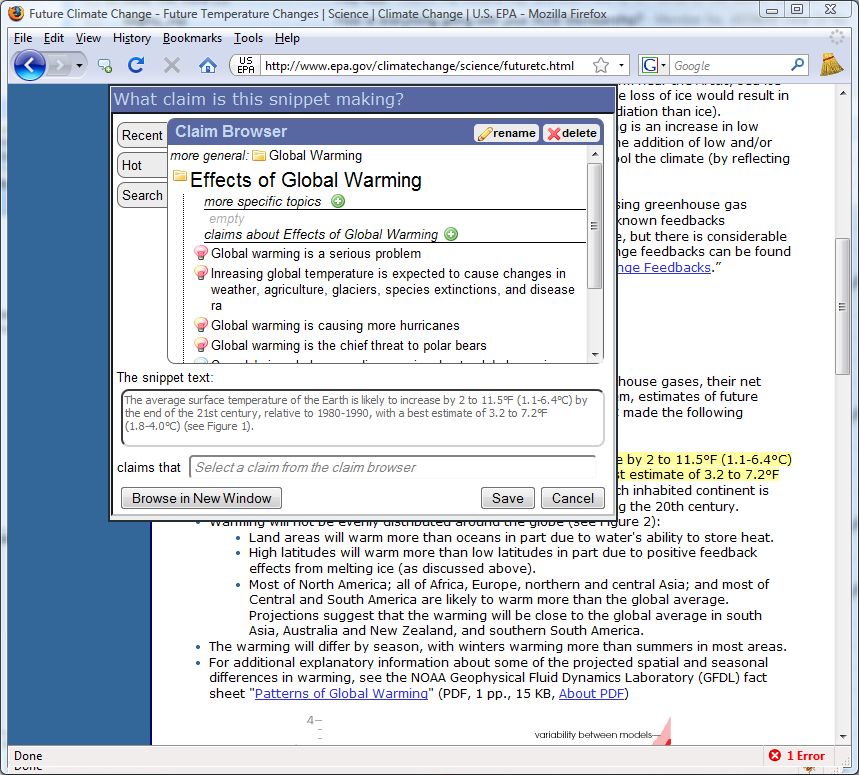
\includegraphics[width=8.5cm]{../screenshots/snipsave_full.png}
%	\caption{The claim selection window allows one to identify the claim a snippet is making}
%	\label{snipsavefull}
%\end{figure}

\begin{figure}[tb]
	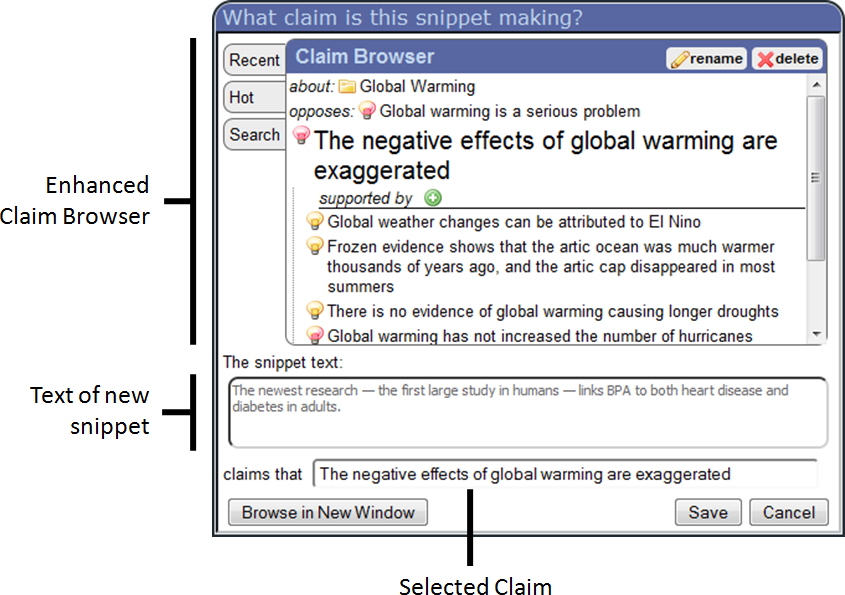
\includegraphics[width=8.5cm]{../screenshots/snipsave_diagram.png}
	\caption{Selecting the claim made by a new snippet}
	\label{snipsavecrop}
\end{figure}


If a user finds a snippet of text on a page that makes an interesting claim then they may want to enter it into Think Link. There are several reasons they may wish to do this. It may be that they find the snippet useful and may want to refer to it again in the future. It may be that they disagree with the claim, and want to alert other readers to the fact that there are opposing arguments, or it may be that they agree with the claim and want to provide easy access to evidence that backs it up. 

To create a new snippet, the user selects the text to be included and then either clicks on the ``new snippet'' button on the browser toolbar, or selects the ``new snippet'' option from the context menu that appears when they click the right mouse button. This is a similar approach to that taken clipping tools such as Google Notebook~\cite{googlenotebook}.

Once the user has identified the text in a snippet, they need to identify the claim that the snippet is making. To do this, Think Link presents the user with a ``claim selection'' window. This window contains a small version of the claim browser that the user can use to select the claim that the snippet is making. At the bottom of the window, we show the phrase ``the snippet text {\it snippet} claims that {\it claim}''. We found that this helps users understand the nature of a claim and its relationship to a snippet.

Since much of Think Link's utility comes from linking snippets together, it is important that to encourage users to reuse existing claims rather than creating new ones, and that when users do create new claims they connect them to existing claims and existing topics. Motivated by this, we designed the claim selection window to make it easier to pick out an existing claim than to create a new one. Moreover, one cannot create a new claim without connecting it to an existing topic or an existing claim. To create a new claim, one navigates to a topic that the claim is about, or a claim that the new claim supports or opposes, and then clicks on the (
\includegraphics[width=0.3cm]{../images/add.png}) button on the list that one wishes to add the new claim to. For example, if the new claim opposes an existing claim, then one clicks the (
\includegraphics[width=0.3cm]{../images/add.png}) button on the ``opposed by'' heading for the existing claim.

This is an intentionally different model to that used by ad-hoc tag-based~\cite{tags} systems such as Delicious~\cite{delicious} and Flickr~\cite{flickr}. This is because in bookmarking or image storing systems it is not so important that duplicates be avoided and that objects be well connected.

In earlier revisions of the interface it was very easy for users to quickly create new claim texts and awkward to find and reuse existing ones. This led users to create many claims that were essentially equivalent and reduced the utility of Think Link as a tool for connection snippets together. 

\todo{Make new snippet icon throb when something is selected}



\subsection{Organizing factual claims}

Much of the value of Think Link comes from the connections between claims. It is thus important that it be easy to establish new connections between claims and topics. 

Think Link uses the familiar drag and drop interface for establishing new connections. To establish a connection between two claims, one need simply drag one claim onto the other. In the full interface, one can open two browsers and drag points from one browser onto points on the other.

In our initial study, we found that many users did not realize that they could use drag and drop to create connections to existing claims. We rectify this, we added a notice at the top of the main organizer window (Figure~\ref{fig:claimbrowser}) telling users that they can use drag and drop.

We found that creating new connections between existing claims was one of the things that users found most difficult.

\todo{say more here}

\section{Discussion}

\subsection{Context of a Claim}

\subsection{How many claims to show}

\subsection{Beyond Claims}

\section{Implementation}

Think Link is implemented as three largely independent components:

\begin{itemize}
\item {\bf A server}, written using Ruby, PHP, and MySQL that maintains a graph of claims, topics, and snippets and provides an API that allows this data to be queried and modified
\item {\bf A web UI}, written using Ruby on Rails~\cite{rails} that provides a visual interface to the claim graph
\item {\bf A page enhancement script}, written in Javascript, that augments the page it is run on by highlighting the factual claims made on the page. This script also provides the ability to create new snippets or display the rails interface to investigate a particular claim.
\item {\bf A browser extension}, implemented for Firefox~\cite{firefoxextension}, that inserts the page enhancement script into all pages the user browses to, and provides toolbar and context-menu shortcuts to the ``new snippet'' feature of the page enhancement script.
\end{itemize}

These components are largely independent. One could use the javascript script on a web page without using the firefox extension, by either manually including it on the page (e.g. to enhance your own blog) or by adding it using a proxy. Since the server API is public, one could write alternative tools that mark up web pages in different ways, or use the claim graph for different purposes.

The source code to Think Link is publicly available under the Apache license at the following URL:

{\b url removed for blind submission}

We expect to have a public deployment available by the time of publication.

We use icons from the free FamFamFam Silk~\cite{silkicons} collection.



\section{User Studies}

We performed two qualitative ``think aloud'' user studies to guide the development of Think Link. 

The aim of the first study was to see how users normally browse the web and how they might go about using Think Link to identify snippets in the pages they browse. The aim of the second study was to evaluate changes made to the interface as a result of the first study and see how people react to browsing pages that have interesting claims highlighted.

\subsection{Procedure for the First Study}

For the first study we recruited 12 paid participants. Five were female, seven were male. Their ages ranged from high school age to retired. Our intention was to recruit users who were not experts, but who regularly used the internet to find information. We recruited participants using a posting to the Craigslist~\cite{craigslist} classified adverts site. In our advert, we expressed an interest in people who use the internet to gather knowledge, rather than just for tasks such as email or shopping. We filtered participants based on their short answers to questions about how they found, organized, and shared information on the web. 

Study sessions took approximately 45 minutes. Participants were seated at a single-screen workstation with the Firefox browser augmented with the Think Link plugin. We first demonstrated Think Link's interface, and then asked them to browse normally and use Think Link to identify snippets that made claims they found interesting and connect those claims to the existing claim graph. For the first half of the study, we asked them to constrain their browsing to political news articles, to increase the likelyhood that there would be existing claims about the topic they were browsing.

In this initial study, users were exposed to the prototype interface shown in Figures~\ref{oldsnippetbox} and \ref{oldbrowser}, rather than the final interface described earlier in this paper. We discuss some of the key differences in the findings section.

\subsection{Procedure for the Second Study}

For the second study, we recruited 6 paid participants. Four were female and two were male. Although we recruited participants using the same advert as the first study, the timing of our second advert around the beginning of the semester meant that five of the participants were students. Since the second group was different demographically to the first group, it was not possible to make a direct comparison between their behaviours. 

In the second study we were more confident about the usability of our tool and so we decided to tell them nothing about how to use it. We gave each user a brief introduction to the aims of the tool, similar to the introduction of this paper, and then asked them to perform two tasks with it. The first task was to look at a selection of web pages that already had highlights and explore the interface while thinking aloud about what they saw. The second task was to identify claims on a set of pages we gave them about global warming and connect them appropriately to existing claims that we had pre-populated our database with. Participants were shown an interface that is largely identical to that described earlier in this paper. 

\subsection{Findings}

In this section we present the findings from our two users studies. Findings from the two studies are presented together and clustered by topic.

\subsubsection{High-Level Impressions}

Response was generally positive, with many participants being very keen to use the tool soon. One partipant said ``I can see myself getting addicted to this'', and several participants asked as to notify them when it becomes publically available. Most of the participants expressed an interest in using the tool, with some wanting to use it now, and others wanting to use it ``when it is more mature''.

Participants liked the ability to see when other pages disagreed with the claim they were looking at. One participant said ``The web needs to be taken with a grain of salt, and this gives you salt goggles''.

\subsubsection{Usability}

Several usability problems were identified with the first version of the tool, causing us to make design changes for the second version. None of these problems re-occured during the second study. We discuss some of these changes in the sections below.

Most participants in the first study, and all participants in the second study were able to use the tool competently. Participants in the second study were able to use Think Link compentently without it being demonstrated in advance and were able to correctly deduce what the different parts of the interface meant. Particpants in the second study said they found the tool ``very intuitive''.


\subsubsection{Browsing the Argument Graph}

%In the first study, several participants reported that they felt ``disorientated'' when browsing through the idea graph.
%
%Several participants in the second study seemed to enjoy the action of browsing through ideas.


\subsubsection{Creating a Snippet}

Users would often encounter a snippet that could be interpreted as making several interesting claims, and were unsure about what to do in such circumstances. Sometimes users would deal with this by writing a compound claim like ``Global Warming will cause X and Y''. While users could mark up the same snippet as making multiple claims, users seemed to find this confusing, suggesting that we may want support in the snippet creation interface for picking several claims that a snippet is making.

One special case of this was that several users wanted to mark up a table as a snippet. A table can usually be considered to be making several interesting claims and users were often confused about what they should say the table cliams. Our current guidance is that one should mark up a table as making the most interesting claims that that table makes. In other cases, a user wanted to mark up an image as a snippet. While Think Link does not currently support this, it might make sense to allow this if an interesting claim can be inferred from the image.

Some users expressed an interest in marking up a snippet as a primary source rather than a claim. For example they might find the text of an important speech or an Olympic results table. Several expressed a desire to have a new class of object that was neither a topic nor a claim, but instead just ``an interesting object relavent to this topic''.

Many users would consistently mark the first paragraph of an article as a snippet. This paragraph would frequently summarise the arguments made in the rest of the document document and often made an important claim that other claims in the document supported or provided context for. 


\subsubsection{Chosing a Claim for a Snippet}

\begin{figure}[t]
	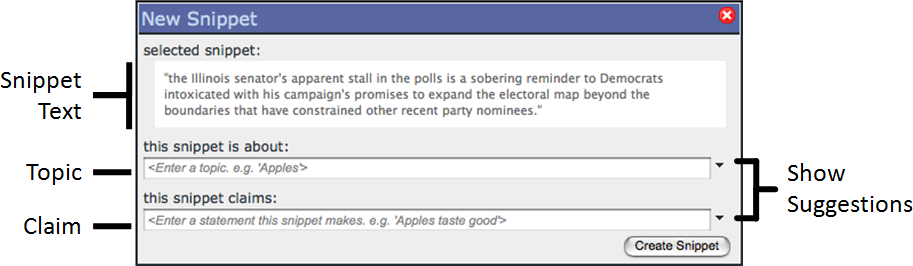
\includegraphics[width=8.5cm]{../screenshots/oldsnipcreate_diagram.png}
	\caption{Initial Prototype Snippet Creation Dialog}
	\label{oldsnippetbox}
\end{figure}

In the initial interface we used a simplified snippet creation window (Figure~\ref{oldsnippetbox}) that was intended to make the process of snippet creation very lightweight. This window contained two text boxes. The first of these boxes was for the topic (e.g. ``Global Warming'') and the second of the boxes was for the claim (e.g. ``Global Warming is Man Made''). Both of these boxes used an auto-complete drop-down list to suggest appropriate existing topics or snippets as the user typed, 
biasing towards topics that were recent or hot. 

We found that participants using this initial interface felt disorientated by the fact that the interface for creating snippets was different to the interface used for visualizing them. Participants would often confuse claims and topics, either entering a claim in the topic box, or a topic in the claim box. Several participants expressed confusion about the difference between the two. Participants would also often create new points and topics when appropriate points and topics already existed in the claim graph, even when the suggestion list was drawing their attention to a topic or claim that would have been appropriate.

For the second study, we used the interface described in Section~\ref{newsnippet}, which uses the same claim browser interface used for exploring the claim graph. We found that users of this interface had no difficulty distinguishing between claims and topics and were much more likely to reuse existing claims and topics. We theorized that part of the reason for increased reuse was that, because users could see the claim graph they were creating, they felt more motivation to keep it ``tidy'' by reusing existing claims.

Several users expressed confusion about how specific the claim made by a snippet should be, or when they should pick an existing claim rather than create a new one. For example, if a snippet says ``Global temperatures will rise by X degrees by 2050'' then is that making the claim ``Global temperatures will rise'', or should a new claim be created that contains the extra information? 

Several users also expressed an interest in being able to use the text of the snippet they selected as the text of its claim, particularly for short snippets. We intentionally made this a little difficult to do in an attempt to encourage users to find existing claims that are appropriate, however this may have been a mistake as it also increases the amount of effort required to create a snippet.

\subsubsection{Connecting Claims}

Many participants expressed a desire to organize claims into connected arguments during their session. 

Some users incorrectly marked one claim as supporting another when in fact they should have both been marked as supporting a third claim that needed to be created, or where an intermediate claim was needed. For example ``Global warming is causing more hurricanes'' does not support ``Global warming is causing rising sea levels'', but both support ``Global warming is causing environmental problems''. Users realized that the claims were related, but did not immediately recognize that they needed to create new claims in order to structure the relationship correctly. It is possible that creating correct logical claim structures may just be too difficult for some people. We hope that, if Think Link was deployed more widely many of the intermediate claims that were needed would already have been created and this problem would be reduced.

Some users were confused by claims that had a ``because'' relationship rather than a ``supports'' or ``opposes'' relationship. For example ``America did not sign the Kyoto Protocol'' {\it because} ``Signing Kyoto would harm the US economy''. Similarly, many users expressed a desire to mark claims as being ``related'' without supporting or opposing each other. For example ``America did not sign the Kyoto Protocol'' {\it is related to} ``America was right to not sign the Kyoto Protocol''. Our current advice in such circumstances is to use topics to group claims that are related. For example these claims could all be in a topic called ``America and the Kyoto Protocol''. Participants seemed comfortable with the idea of relating claims in this way when we pointed it out to them, but most participants needed to be told that this was a strategy they could use.

Several users got confused by claims that referred to similar events at different points in time. For example, one participant in the first study marked a two claims as opposing each other when each was true at the time that it was written. This is a particular problem when talking about breaking news events, where what claims are true can change fast. If Think Link is to be effective for describing such events then it is likely that it will need to have better support for identifying the {\it time} at which a claim was asserted to be true.

Several users expressed an interest in being able to mark a claim as contraversial without having to create an opposing claim. One user said that opposing a claim required ``too many clicks'' and they wanted to be able to just vote against a claim without having to say why or find evidence. In the future we are planning to implement a social voting system to allow users to say what claims they believe are false and see what claims their friends agreed or disagreed with.

\begin{figure}[ht]
	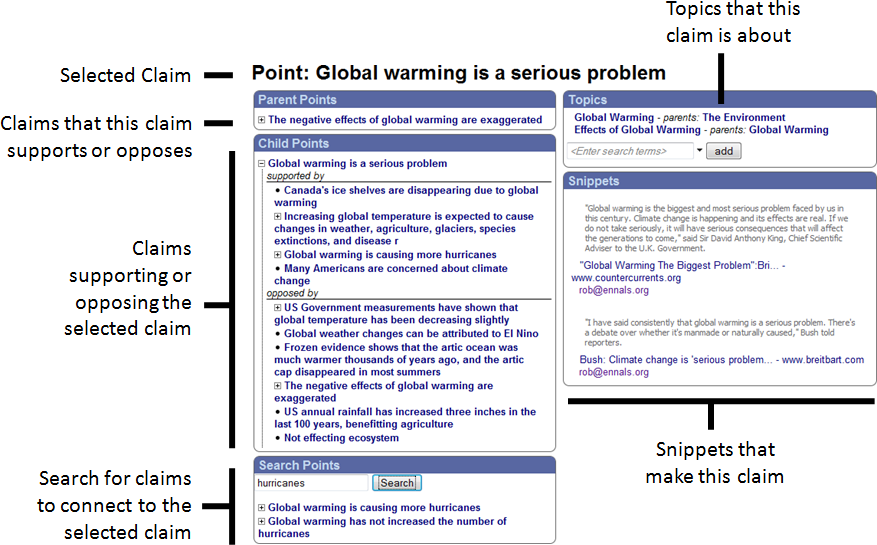
\includegraphics[width=8.5cm]{../screenshots/oldpoint_diagram.png}
	\caption{Initial Prototype Claim Browser}
	\label{oldbrowser}
\end{figure}


\section{Limitations and Future Work}

There are a number of issues that a widely released tool would need to address. Firstly, our current implementation has privacy issues. Every time one navigates to a web page, the plugin contacts our server and gives it the current URL so that it can check if there are snippets on that page. This information is anonymous, cacheable, and not logged, but it is still likely that some people would object to this information being given to an external server. 

At present, all claims have to be marked up by users who must not only identify the correct section of text to highlight, but also use a browsing interface to find the interesting claim that is being made. It would be interesting to see if natural language processing techniques could be used to either simplify the process of marking snippets, or even to detect snippets that make known claims without human intervention.

While Think Link is influenced by Wikis, it does not currently have support for reverting bad edits made by previous users, or managing history in general. It will be interesting to see what interfaces work well for managing history, given that our data is a graph rather than a series of pages.

Similarly, Think Link is designed to be used as a social tool in which large numbers of people collaborate to find large numbers of claims and snippets about interesting topics. Since our graph and user base are currently small we have not yet evaluated how Think Link works when data sets are huge, many users are concurrently editing data, and some users are malicious.

We think it could be useful to use Think Link as a tool to suggest reading material. Just as tools like Digg suggest pages that you might like, Think Link could potentially suggest pages that contain claims that the user had not read and would be likely to find interesting.


\section{Conclusions}

We have introduced the concept of browsing the web of factual claims using Think Link. Think Link allows users to navigate between pages based on the factual claims made on pages, rather than being restricted to the links provided by authors. It allows users to identify contentious claims on web pages and connect them directly to the arguments that those claims are part of, and related claims on other web sites.

On a practical level, Think Link works by allowing users to pick out snippets on pages that make claims that they think are interesting or contraversial, and then using a wiki model to allow users to collaborate together to structure claims into an argument graph.

We hope that Think Link will make it easier for people to be informed about the world and be exposed to factual claims that they might not otherwise be exposed to.

\section{Acknowledgements}

We would like to think Allison Woodruff, Tye Rattenbury, and all our user study participants for all their help during the design of Think Link.


\bibliographystyle{abbrv}
\bibliography{biblio}

\end{document}
